\documentclass [12pt]{beamer}

\usepackage{algpseudocode} 
\usepackage{algorithm2e} 
\usepackage[utf8]{inputenc}

\author{Jake Humphrey}
\title{Une Approche de Calcul Stochastique pour l'Evaluation de Fiabilité Précis et Efficace}
\subtitle{Une Implementation Python}
\institute{Department of Electronic and Electrical Engineering\\
  Imperial College London\\
  \texttt{jbh111@ic.ac.uk}
}

\begin{document}

\begin{frame}[plain]
  \titlepage
\end{frame}

\begin{frame}{Fiabilité des Circuits}
Des Portes dans un circuit logique sont sensibles aux erreurs:
\begin{itemize}
\item \textbf{Erreur Coincé-A-Un:} La sortie va haute.
\item \textbf{Erreur Coincé-A-Zero:} La sortie va basse.
\item \textbf{Erreur Von Neumann:} La sortie est inversée.
\end{itemize}
\end{frame}

\begin{frame}{Effets de masquage}
Cependant, il est possible que l'erreur n'affecte pas la sortie en raison de l'un des \emph{effets de masque} suivants:
\begin{itemize}
\item \textbf{Masquage Electrique:} Signal d'erreur trop faible pour être détecté.
\item \textbf{Masquage Temporel:} Erreur manque la fenêtre de détection d'un latch.
\item \textbf{Masquage Logique:} L'erreur ne modifie pas la sortie d'une porte logique.
\end{itemize}
\end{frame}
\begin{frame}{Analyse de Fiabilité \small Principes}
Masquage logique est le plus commun, et on essaye d'analyser des circuits sur leur capacité à masquer logiquement des erreurs.
\vspace{0.25cm}

\emph{Probabilité} d'un signal = Chance qu'il est logiquement vrai.

\emph{Fiabilité} d'un signal = Chance qu'il prend la valeur correcte.
\vspace{0.25cm}

Puis:
\begin{itemize}
\item Construire une représentation défectueux du circuit.
\item Dériver les \emph{probabilités} des sorties à partir des entrées.
\item Trouvez les \emph{fiabilités} des sorties.
\end{itemize}
\end{frame}

\begin{frame}{Analyse de Fiabilité \small Modèles de Portes Probabilistes}
\only<1>{
Cependant, les algorithmes existants sont inefficaces!
\vspace{0.25 cm}

Par exemple, les \emph{Modèles de Portes Probabilistes} ( En Anglais \emph{Probabilistic Gate Models}, PGMs) tenter de dériver les probabilités de sortie de façon déterministe et analytique.
}
\only<2>{
Le problème se produit lorsque les entrées à une porte sont statistiquement dépendante.
\vspace{0.25 cm}

Les équations PGM ne tiennent pas compte des signaux statistiquement dépendantes, et la solution exige que le circuit soit divisé en deux sous-circuits, qui double le coût de l'algorithme.
}
\end{frame}

\begin{frame}{Analyse de Fiabilité \small Calcul Stochastique}
L'utilisation de \emph{Calcul Stochastique} peut éviter ces problèmes.
\vspace{0.25 cm}

Générez des flux binaires d'entrée et les propagez à travers le circuit.
\vspace{0.25 cm}

Les probabilités de sortie peuvent ensuite être calculés avec précision à partir des flux de bits de sortie.
\end{frame}

\begin{frame}{Analyse de Fiabilité \small Calcul Stochastique avec des Suites Bernoulli}

Algorithmes existants de calcul stochastique utilisent les probabilités d'entrée pour générer des \emph{Suites Bernoulli} de la forme:

\begin{equation*}
[X_0, X_1 \dots X_{n-1}]; X_i \sim B (p)
\end{equation*}

pour chaque entrée, où $p$ est la probabilité d'entrée.
\vspace{0.25 cm}

Nécessite que $n$ nombres aléatoires doivent être générés pour chaque entrée!
\end{frame}

\begin{frame}{Analyse de Fiabilité \small Calcul Stochastique avec les Suites non-Bernoulli}
\emph{Suites non-Bernoulli} réduisent le coût en raison de génération de nombres aléatoires.
\vspace{0.25 cm}

Ils sont générés de manière déterministe avec l'espérance des 1s, puis permutées au hasard.
\vspace{0.25 cm}

Seulement une génération d'une nombre aléatoire est requis par flux binaire d'entrée!
\end{frame}

\begin{frame}{Algorithme d'Analyse de la Fiabilité}
En utilisant le calcul stochastique avec les suites non-Bernoulli, on arrive à un algorithme pour analyser de fiabilité, que je vais décrire dans les diapositives suivantes.
\end{frame}

\begin{frame}[fragile]{Algorithme d'Analyse de la Fiabilité \small Pseudocode}
\begin{algorithm}[H]
\KwData{circuit logique à tester}
\KwResult{fiabilités pour chaque sortie}
\For{chaque porte dans le circuit}{représenter porte dans le circuit défectueux\;}
\For{chaque entrée du circuit défectueux}{générer une suite non-Bernoulli\;}
\For{chaque sortie dans le circuit}{
\For{chaque vecteur d'entrée}{
\If{les sorties sont les mêmes pour chaque circuit}{ajouter 1/n à la fiabilité de sortie \;}
}
}
\end{algorithm}
\end{frame}

\begin{frame}{Algorithme d'Analyse de la Fiabilité \small Analyse de la Complexité}
La section la plus coûteuse est la double boucle finale!
\vspace{0.25 cm}

Il faut propager un signal à travers chaque circuit une fois pour chaque sortie, et $n$ fois.
\vspace{0.25 cm}

Peut-être, au pire, $O(ogn)$, où:

$o$ = nombre de sorties

$n$ = longueur de suites non-Bernoulli

$g$ = nombre de portes
\end{frame}

\begin{frame}[fragile]{Algorithme d'Analyse de la Fiabilité \small d'Autre Travail}
Il y a encore place à l'amélioration: les entrées se propagent à travers le circuit une fois par sortie.
\vspace{0.25 cm}

Il doit recalculer de nombreuses valeurs intermédiaires redondantes!
\vspace{0.25 cm}

Calculer toutes les valeurs de sortie une seule fois permettrait de réduire la double boucle à un seul sur la longueur des séquences d'entrée.
\vspace{0.25 cm}

Ceci réduit la complexité de l'algorithme à $O(gn)$
\end{frame}

\begin{frame}{Algorithme d'Analyse de la Fiabilité \small Analyse d'Exécution}
\center
\only<1>{
\begin{tabular}{l | r r}
Fichiers d'entrée & c17.v & c432.v \\
   \hline
   Entrées & 5 & 36 \\
   Sorties & 2 & 7 \\
   Portes & 6 & 160 \\
   \hline
   Longeur de la Suite d'Entrée & runtime /s & runtime /s \\
   \hline
   1 & 0.00023 & 1.34 \\
   10 & 0.00067 & 12.2\\
   100 & 0.00485 & 122 \\
   1 000 & 0.0473 & 1 250 \\
   10 000 & 0.458 & Aucune donnée\\
   100 000 & 4.66 & Aucune donnée
\end{tabular}}
\only<2>{
\begin{figure}
   \centering
     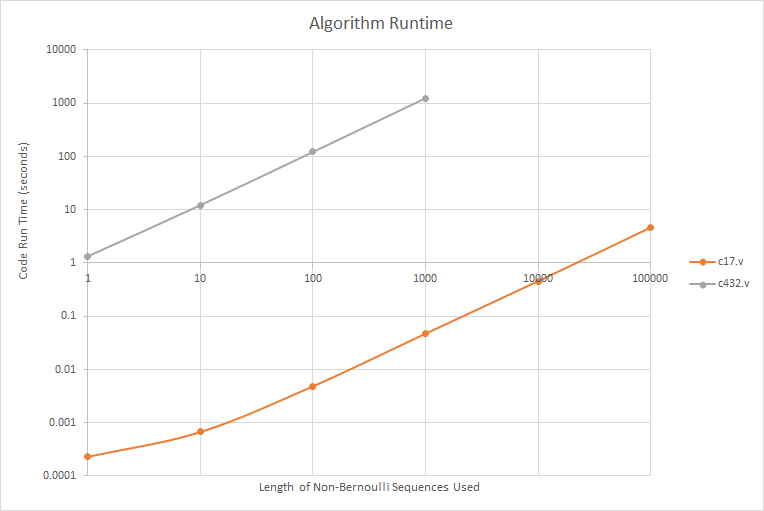
\includegraphics[width=\textwidth]{runtime}
\end{figure}
}
\end{frame}
\end{document}